
\documentclass[conference]{IEEEtran}

\ifCLASSINFOpdf

\else

\fi
\onecolumn

\usepackage{amsmath}
\usepackage{fancyvrb}
\usepackage{float}
\usepackage{verbatimbox}
\usepackage{graphicx}
\usepackage{float}

\begin{document}

\title{Matrix Multiplication Using MapReduce}

\author{\IEEEauthorblockN{Arlo Eardley (1108472), Carel Ross (1106684) and Ryan Verpoort (1136745)}
\IEEEauthorblockA{School of Electrical and Information Engineering, University of the Witwatersrand, Johannesburg 2050, South Africa}}

\maketitle
\thispagestyle{plain}
\pagestyle{plain}

\IEEEpeerreviewmaketitle

\section{Overview}

\noindent The work conducted involves the use of the MapReduce framework which is used for processing large amounts of data. The framework also uses computational techniques that are reliable and fault-tolerant. The MapReduce framework usually consists of the following three operations:

\begin{enumerate}
\item \textbf{Mapping:} Big data is distributed into sub-tasks and executed by workers, while being coordinated by a master task, with output keys being generated during this step
\item \textbf{Shuffling:} Based on the output keys, workers redistribute data so that all data related to a key is being operated on by the same worker
\item \textbf{Reducing:} Workers perform the sub-tasks, process each group and then merge the values into the final result
\end{enumerate}
\medskip
\noindent The Mrs-MapReduce framework is used in this investigation with the aim of determining the product of two matrices A and B such that:
\[C = A \times B\] 

\noindent Two different algorithms are implemented to achieve the matrix multiplication, namely the iterative and the divide and conquer approaches. The MapReduce procedure is further described as a parallel and distributed computation such that:\\

\begin{itemize}
\item The map procedure assigns each task to an input key value. The task then receives the data associated with the corresponding input key value.
\item Map runs for each input key value and generates a corresponding output key value.
\item The output pairs are then "shuffled" to assign task to these pairs.
\item For each output pair, the reduce procedure is run.
\item The output from the reduce procedure is collected and organized by the output pairs. This is then the final result.
\end{itemize}

\section{Input}

\noindent The matrix format will be as follows for a particular matrix:\\
\begin{equation*}
A[3][4] =
\begin{bmatrix}
a       &b      &c      &d\\
e       &f      &g      &h\\
i       &j      &k      &l\\
\end{bmatrix}
\end{equation*}

\noindent With data stored in a text file in the following format:

\begin{equation*}
\begin{matrix}
3       &4      & \\
0       &0      &a\\
0       &1      &b\\
1       &2      &l\\
0       &3      &d\\
1       &0      &e\\
2       &0      &i\\
1       &1      &f\\
1       &2      &g\\
2       &1      &j\\
0       &2      &c\\
2       &2      &k\\
1       &3      &h\\
\end{matrix}
\end{equation*}

\noindent The data is then manipulated and processed for each corresponding algorithm. The input will divide the data into appropriate sizes and the data will then be assigned to each map function. In this case this process is done by reading each line from a text file as a record to be processed by the map function.\\

\section{Mapping}

\noindent The map function receives an input of key/value pairs, where each worker node applies the map function to these pairs. The master node manages the input data, so that no process is run twice. The number of maps is usually the equal to the number of input records. The input key/value pairs are processed and mapped to a series of output key/value pairs. The input pairs will map to zero or multiple output pairs. For example, the key/value pairs within a matrix consist of the position of a value within a matrix as the "key" and the value at that position as the "value". These will then be mapped to an output key/value pair to be manipulated in the reduction phase. This can be seen in Fig. 1. below:

\noindent
\begin{figure}[H]
\centering
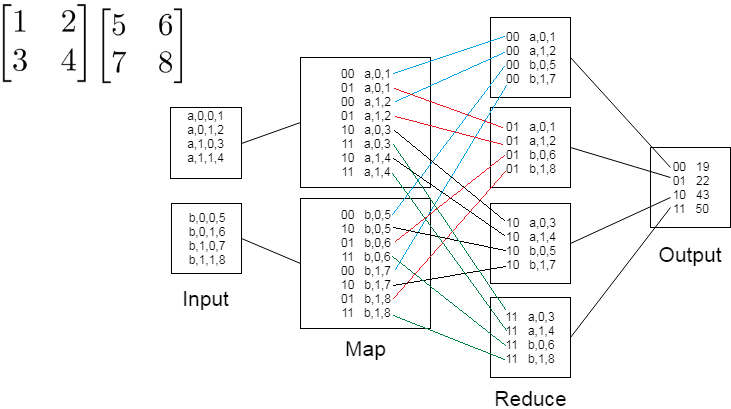
\includegraphics[width =\linewidth]{MapReduce2.png}
\caption{A diagram of the mapping procedure}
\label{fig:circuit}
\end{figure}

\section{Reducing}

\noindent The reduce function is called once for every unique key. The reduce function consists of three phases namely Shuffle, Sort and Reduce. The output keys from the map function are "Shuffled" using a parallel sorting method to distribute the keys to the desired reducer. The data needs to be approximately uniformly distributed so that the operation does not need to wait for reducers that have been assigned more operations. The worker nodes process the output pairs, in parallel, after they have been sorted. These output pairs consist of a smaller set of values which share a key, as shown in Fig. 1. The reduce function does the corresponding calculation for each of the output pairs and generates the output values. There are usually less reduce jobs than map jobs. It is also viable to have no reduce jobs if required.\\ 

\section{Output}

\noindent The output matrix format will be as follows for a particular matrix:

\[A[3][4] \times B[4][3] = C[3][3]\] 
\begin{equation*}
C[3][3] =
\begin{bmatrix}
a       &b      &c\\
d       &e      &f\\
g       &h      &i\\
\end{bmatrix}
\end{equation*}

\noindent After the calculation has been reduced the matrix output is determined and written to stable storage, within the computer, in the following format:

\begin{equation*}
\begin{matrix}
3       &4      & \\
0       &0      &a\\
0       &1      &b\\
0       &2      &c\\
1       &0      &d\\
1       &1      &e\\
1       &2      &f\\
2       &0      &g\\
2       &1      &h\\
2       &2      &i\\
\end{matrix}
\end{equation*}

\section{Algorithm A (Iterative Approach)}

\noindent This algorithm implements an iterative approach to matrix multiplication. The product of matrix A and matrix B can be determined by evaluating the dot product of the two matrices. This means that A * B = C, where matrix C is the product of matrix A and B. The map function will use the input and map each of the key/value pairs of every element of the matrix and is repeated for both input matrices. The reduce function then takes every mapped function and multiplies and adds the corresponding key values to return the final result. Fig. 2. below demonstrates this concept.  


\noindent
\begin{figure}[H]
\centering
\includegraphics[scale=0.6]{StandiMultiplication.png}
\caption{Matrix multiplication using iterative approach}
\label{fig:circuit}
\end{figure}




\section{Algorithm B (Divide And Conquer Approach)}

\noindent This algorithm implements a divide and conquer method. The product of matrix A and matrix B can be determined by evaluating the dot product of the two matrices. This means that A * B = C, where matrix C is the product of matrix A and B. The map function will use the input and map each of the key/value pairs of every element of the matrix and is repeated for both input matrices. The map function will generate two key/value pairs for the same input record as shown in Fig. 3. below, since the a value in matrix A is used in both the first and second column of the evaluation in matrix C. This means that all row values from matrix A will be in every row of matrix C, as well as all column values will be in every column of matrix C. During the reduction phase the values with the same keys are grouped and multiplied according to their row/column value as shown in Fig . 3. . These new values are then summated and positioned in matrix C based on their key value.\\

\noindent
\begin{figure}[H]
\centering
\includegraphics[scale=0.6]{DivideAndCon.png}
\caption{Matrix multiplication using Divide and Conquer approach}
\label{fig:circuit}
\end{figure}
  
 
\section{Graph Theory}

\noindent A method used to determine the result of matrix multiplication is to use a directed graph G such that G = (v, e). Where v is the number of nodes and e is the number of edges of the graph. For example: node A and B are directly connected via a single edge of a particular length. If all edges in the graph are of the same length then it is an un-weighted directed graph, as seen in in Fig. 4. . Matrix multiplication can be achieved through the use of graphs and this process is represented in Fig. 4. and described as follows:\\

\begin{enumerate}
\item A node represents an index value in the matrix. For example in Fig. 4. node 0 refers to the index 0 of the matrix.
\item An edge joins two nodes with the length of the edge directly corresponding to the value in the matrix, if the length is 0 then there is no edge.
\item The matrix can be mapped by using the indexes and values at those indices.
\end{enumerate}

\medskip
\noindent For example, using Fig. 4., the value M\textless i, j\textgreater = M\textless 0, 2\textgreater = 1 can be transformed into a directed graph by having a directional edge of length one from node zero to node two. This process is repeated until the entire graph is mapped. It is also possible for an edge to have the same source and destination node.
Once the graph is mapped, M\textsuperscript{K}\textless i, j\textgreater can be determined by using the desired source node (the corresponding matrix index i) and summing the number of possible K-step routes to get to the destination node (the corresponding matrix index j), while following the directional edges. Since the graph is directional, no redundancies occur. This means that when using the MapReduce framework to determine the matrix M\textsuperscript{3}, then the summation of all values in the resulting matrix will be the total number of pairs of nodes that are connected by a path of length 3 in matrix M. The number of ways that a pair of nodes are connected by a path of length 3, can be determined by using the value in the matrix at the corresponding node indices. Fig. 4. also shows how matrix multiplication can relate to road networks or power transmission lines, by using this mapping technique in conjunction with the MapReduce framework.
  
\noindent
\begin{figure}[H]
\centering
\includegraphics[scale=0.4]{MTXMultiplication.png}
\caption{Matrix Multiplication}
\label{fig:circuit}
\end{figure}



\section{Results}
\noindent The implementation of the two algorithms, to solve the matrix multiplication problem, results in the divide and conquer method being more focused on the mapping procedure and the iterative method being more focused on the reduction procedure. Table I below displays the results from the  two algorithms run for various matrix sizes. The divide and conquer method is consistently slower than the iterative approach due to the aforementioned reliance on the mapping procedure. 


\begin{table}[H]
\centering
\caption{A table of Results for the matrix multiplication} 
\begin{tabular}{|c|c|c|c|c|}
\hline
Size classification             &Matrix size A      & Matrix size B         & Algorithm                 & Total Time (s)\\
\hline
Small                           &20 x 20            &20 x 20                &Iterative                  &0.051\\
\hline
Small                           &20 x 20            &20 x 20                &Divide and Conquer         &0.200\\  
\hline
Medium                          &200 x 200          &200 x 200              &Iterative                  &9.722\\
\hline
Medium                          &200 x 200          &200 x 200              &Divide and Conquer         &150.190\\
\hline
\end{tabular}

\end{table} 

\noindent  A limitation of the implementation is that it is only able to perform using integer values within the matrices. There is also limited error checking and it is therefore a requirement for the number of columns of matrix A to equal the number of rows of matrix B in order to calculate the matrix multiplication correctly. Within the output file of \textit{AlgorithmA}, the output matrix indices and corresponding values are between the parentheses. The preceding value is the number of keys used during the reduction phase of the algorithm. The output file of \textit{AlgorithmB} only shows the output matrix indices and the corresponding values.

\newpage
\section{Pseudo-Code}
\subsection{Iterative}
\begin{verbatim}

class MatrixMultiply():

    def map():
    
        for line in textfile:
            word = remove spaces in line
		
            if length of word == two:
            set which file is currently being used
			
                if file is matrix A:
                    store both matrix dimensions
				
                if file is matrix B:
                    store number of columns
				
            if length of word == three:
		
			    store matrix indices and their values
			
            if there are still lines in textfile:
            
                if file is matrix A:
                    yield map values for iterative 
                if file is matrix B:
                    yield map values for iterative

    def reduce():

	    output = initialize array of zeros
	
        for i values:
            split i into row and column values
		
            if file is matrix A:
                store row and column values matrix A
            if file is matrix B:
                store row and column values matrix B
			
        sort both matrices according to row and column values
        
        if length of matrix A == matrix A rows and length of matrix B == matrix B columns:	
    	
            for i values in rows:
                for j values in columns:
                    for k values in Matrix A columns:
                    
                        multiply and add values for matrix multiplication
                    yield indices with final result

if main function:
    run script
    
\end{verbatim}


\subsection{Divide and Conquer}
\begin{verbatim}

class MatrixMultiply()

    def map()
    
        for line in textfile
        
            word = remove spaces in line
		
            if length of word == two:
                store values of matrix dimensions
			
            if length of word == three:
                store matrix indices and their values
			
            if there are still lines in textfile:
			
                if file is matrix A:
                    for keys in column:
                        yield map values for divide and conquer
						
                if file is matrix B:
                    for keys in row:
                        yield map values for divide and conquer

    def reduce():
    
        for k values in columns:
            make sets of corresponding values 
		
        for k values in columns:
            perform multiplication
		
        yield final summated result

if main function:
    run script

\end{verbatim}


% that's all folks
\end{document}


